\documentclass[english]{paper}


%%%%%%%%%%%%%%%%
%---PACKAGES---%
%%%%%%%%%%%%%%%%
\usepackage[T1]{fontenc}
\usepackage[latin9]{inputenc}
\usepackage{geometry}
\geometry{verbose,tmargin=3cm,bmargin=3cm,lmargin=2cm,rmargin=2cm,headheight=2cm,headsep=2cm,footskip=2cm}
\usepackage{float}
\usepackage{graphicx}
\usepackage{multicol}
\usepackage{hyperref}
\usepackage{babel}
\usepackage{natbib}
\usepackage{booktabs}
\usepackage{multirow}

%%%%%%%%%%%%%%%%%%%%%%%%%%%%%%%%%%%%%
%---USER SPECIFIED LaTeX COMMANDS---%
%%%%%%%%%%%%%%%%%%%%%%%%%%%%%%%%%%%%%

\makeatletter

\newenvironment{lyxcode}
{\par\begin{list}{}{
\setlength{\rightmargin}{\leftmargin}
\setlength{\listparindent}{0pt}% needed for AMS classes
\raggedright
\setlength{\itemsep}{0pt}
\setlength{\parsep}{0pt}
\normalfont\ttfamily}%
 \item[]}
{\end{list}}

\graphicspath{{figures/}}

% or sth else
\def \spreadname {SpreaD3}

\makeatother

%%%%%%%%%%%%%%%%
%---DOCUMENT---%
%%%%%%%%%%%%%%%%

\begin{document}

\title{{\spreadname}: Spatial Phylogenetic Reconstruction of Evolutionary Dynamics 3}
\maketitle

\begin{flushleft}
\textbf{Authors}
\par\end{flushleft}

\noindent
Filip Bielejec (\url{filip.bielejec(sorry_spybots)rega.kuleuven.be}) \\
Guy Baele (\url{guy.baele(sorry_spybots)rega.kuleuven.be}) \\
Bram Vrancken  (\url{bram.vrancken(sorry_spybots)rega.kuleuven.be}) \\
Marc Suchard (\url{msuchard(sorry_spybots)ucla.edu})\\
Andrew Rambaut (\url{a.rambaut(sorry_spybots)ed.ac.uk}) \\
Philippe Lemey (\url{philippe.lemey(sorry_spybots)rega.kuleuven.be}) \\

\begin{flushleft}
\textbf{Contact}
\par\end{flushleft}
Filip Bielejec (filip.bielejec@rega.kuleuven.be) 


\begin{flushleft}
\textbf{Download}
\par\end{flushleft}
SpreaD3 and its source code are freely available from \url{https://github.com/phylogeography/SPREAD2}.
You can also clone the project with Git by running: 
\\\$ git clone https://github.com/phylogeography/SPREAD2. (TO DO: change name to SpreaD3)
\\
cd into the base dir and compile SpreaD3 by running 
\\\$ ant jar
\\
This builds a executable jar-file in the directory ./dist, which can be run by double-clicking it.
%All data used in the examples (cfr. infra) are available from \url{https://rega.kuleuven.be/cev/ecv/software/SpreaD3}.

%---TOC---%
\pagebreak{}
\tableofcontents{}
\pagebreak{}

\section{Introduction}
% 1. Intro
% - Spread is 2-step analysis now 
% - we use JSON as a medium for the pipeline
% - a word of explanation what is JSON notation, how it can be read by
%   any O-O language (python, JS)
% - D3 (what it is etc), what is GEOJSON, how we use it as canvas for our
%   vis, where to get it from, maybe a couple of tips on manipulating
%   GeoJSON files (there are tools to merge, split etc).
% => created separate section for this - software requirements 

% - still some support for KML and GE

SpreaD3 is major rewrite of SPREAD \citep{bielejec11}, a tool for analysing and visualising discrete and continuous trait evolutionary histories associated with phylogenies.
It is designed primarily for use in conjunction with the popular Bayesian phylogenetics software BEAST \citep{drummond:2012zr}.
%These phylogenies are usually temporally resolved, but can also have branch lengths measured in nucleotide substitutions.
%BEAST style annotated file
%To cover both single tree summaries as well as collections of plausible histories (trees), 
%The program is designed to parse BEAST style annotated trees, and thus 
However, it can also accommodate input generated by other phylogenetics inference tools (e.g. MrBayes and BEAST2 or maximum likelihood approaches) as long as the nodes and branches are commented using the appropriate syntax.
\par
The user is offered great flexibility in and control over the visualisation process through two main innovations.
First, each analysis is conceived as a two-step process. 
%separating the parsing and rendering steps
%to maximise flexibility in the visualisation process without a need for the repeated parsing of input data. 
At the parsing step the input is converted to a JavaScript Object Notation (JSON) compliant data file.
Nodes are translated to points, branches to lines and both can have associated annotations. 
Next, the JSON formatted output is used for rendering the visualisations.
By separating the parsing from the rendering, the user can quickly test various image setups without the need for repeatedly parsing the same input.
Note that because JSON is a language-independent data format, the output of the parsing step can be forked to utilities based on several programming languages through dedicated packages and libraries. %examples?
Second, much of the added versatility from this version comes from the newly introduced capability of combining several layers in one illustration. %, as has become default in all widely-used image editors (e.g. Adobe CS, ???).
On the one hand this lifts the restriction of projecting phylogenies on a pre-specified canvas, and gives the user detailed control on the type of map and the displayed %geographical 
attributes (e.g. province borders, altitude contours, population density, \dots). %or no examples? .
At the same time this opens door to mapping traits using any arbitrary coordinate system (see \ref{tips} for an example). 
%are a number of default maps provided? I.e. a world map? where can such input be found? 
A third advantage of the layered approach to image building is the ease with which complex stratified images can be constructed (see \ref{JSONmerge} for an example). 
\par
Alongside enhancing the flexibility in creating the visualisations, the other prime objective of SpreaD3 is to drastically facilitate the on-line publishing of interactive visualisations.
This is achieved by rendering the figures using the Data Driven Documents JavaScript libraries (D3, see \url{www.d3js.org} and \citet{Bostock:2011aa}) to project the annotated phylogenies on a map in geoJSON data structure format (\url{www.geojson.org}).
%how can a longitude/latitude globe reference easily be converted to the corresponding coordinates on a geoJSON map? 
%how can the latter easily be constructed (geojson.io? https://google-developers.appspot.com/maps/documentation/utils/geojson/?)
For reasons of consistency with the previous version, and as an illustration of the branching to other renderers enabled by the versatile JSON data format as a go-between, SpreaD3 also supports re-interpreting parsed input data in the Keyhole Markup Language (KLM) for visualisations in virtual globe software like Google Earth (\url{www.google.com/earth/}). 
\par
In this tutorial we give a detailed description of program functionalities, with an emphasis on the Graphical User Interface (GUI), by presenting an example for the main genres of possible analyses and give general guidelines on running SpreaD3. 
The data files used in the example can be found at  \url{https://rega.kuleuven.be/cev/ecv/software/SpreaD3}.
The user is assumed to know how to build a Maximum Clade Credibility (MCC) tree. 
A good tutorial on how to summarize BEAST trees with TreeAnnotator can be found at \url{???}.

\section{Software requirements}

\section{geoJSON maps}

There are many places where ready-made geoJSON maps are available, and various ways in which tailor-made geoJSON maps can be made. 
We point out a few resources, but don't even attempt to provide an exhaustive list.
\\
A good introduction to building geoJSON maps can be found here: \url{http://bost.ocks.org/mike/map/}.
Large repositories for geoJSON maps can be found here:
\url{http://grokbase.com/t/gg/d3-js/1372gq18j9/geojson-maps} and \url{http://data.okfn.org/data/datasets/geo-boundaries-world-110m}.
% and \url{http://geocommons.com/}.
\\
There are a number of easy-to-use utilities for creating geoJSON maps starting from shape files. 
The latter can be among others found at \url{http://www.naturalearthdata.com/downloads/} and \url{http://www.gadm.org/}.
An example of a conversion utility is \url{http://www.mapshaper.org/} or its command line version available at \url{https://github.com/mbloch/mapshaper}.
\par
A handy feature is that the latitude and longitude are treated as absolute values in the geoJSON format.
Like this, the coordinates for a location (e.g. Leuven) remain valid when providing a more focused map (e.g. Belgium instead of the entire world).
If no geoJSON map is provided, a bounding box based on the provided coordinates will be created automatically.

\section{Usage examples}

SpreaD3 can process four distinct input types labelled MCC tree with DISCRETE traits, Log file from BSSVS analysis, MCC tree with CONTINUOUS traits, Tree distribution with CONTINUOUS traits. 
These specify the basic type of analysis performed, with more options available by selecting different parser options for a given input.
% 
% 2. Examples of usage. Whese should show not just how but also why, what
% can we learn by visualising these processes.
% 
\par
For the command line examples throughout this tutorial we assume the following alias has been added to your .bash\_profile:
\\
alias spread=`java -jar <absolute path to SpreaD3.jar>' 
\\
The alias will become active when you open another session in Terminal, or it can be used in the current session after executing
\\
\$ source $\sim$/.bash\_profile
\\
in the current session  [\#assuming your bash\_profile resides at \$HOME]. 

\subsection{Visualizing a MCC tree annotated with discrete traits}
% 
% 2.1 MCC tree with discrete traits.
%  - Here we could use the EBOV as a case for study. All the steps Parse
% -> render -> manipulate the visualisation, screenshots etc. Place live links to data (hosted at github)   

In this example we turn to the recent Ebola virus outbreak in western Africa to show how a MCC tree summary created under a discrete diffusion model \citep{lemey:2009fk} can be used to visualise its spatiotemporal spread. 
Samples were collected from March to December 2014; BEAST \citep{drummond:2012zr} was used to co-estimate the temporal and spatial history. 

\subsubsection{Parsing the data}
The GUI opens in the `Data' tab.
Select the option `MCC tree with DISCRETE traits' (Figure \ref{fig:parseDiscrete}, nr.1), and browse to where you saved the example MCC tree to load it.
SpreaD3 will now set the working directory to the one from which the MCC tree was loaded. 
This means that all output generated by SpreaD3 will be saved in this directory.
To view the MCC tree in its geographic context, we have to associate each location with a particular latitude and longitude. 
To do this, indicate under which name the location trait is known (Figure \ref{fig:parseDiscrete}, nr.2) and associate the appropriate coordinates with each location.
For this you can either use the editor supplied with SpreaD3 (Figure \ref{fig:parseDiscrete}, nr.3) or load a previously prepared tab-delimited file including each location, its latitude and longitude. 
\par
SpreaD3 sets the most recent sampling date to the current date. 
In this example, the date should be set to 27/12/2014 (Figure \ref{fig:parseDiscrete}, nr.4).
Leave the `Time scale multiplier' (Figure \ref{fig:parseDiscrete}, nr.5) to its default value of 1 \footnote{This option is useful when the time units should be rescaled,  e.g. in molecular archeological work}. 
Next, browse to the location where the geoJSON file is stored and load it (Figure \ref{fig:parseDiscrete}, nr.6).
The number of intervals equals the number of periods in which the history is partitioned (Figure \ref{fig:parseDiscrete}, nr.7). %correct?
Specifically, all lineages of the tree are virtually intersected at each transition time and the the number of branches over which no trait state transition has occurred (e.g. no change in location between the branch's parent and child node) contribute to the trait's Markov reward counts at that time slice.
The reward counts (`Circular polygons', cfr. infra) at slice $n$ are plotted in the animation starting from period $n$.
Save the file as `ebov.json' (Figure \ref{fig:parseDiscrete}, nr.8).

\begin{figure}[!H]
\centering
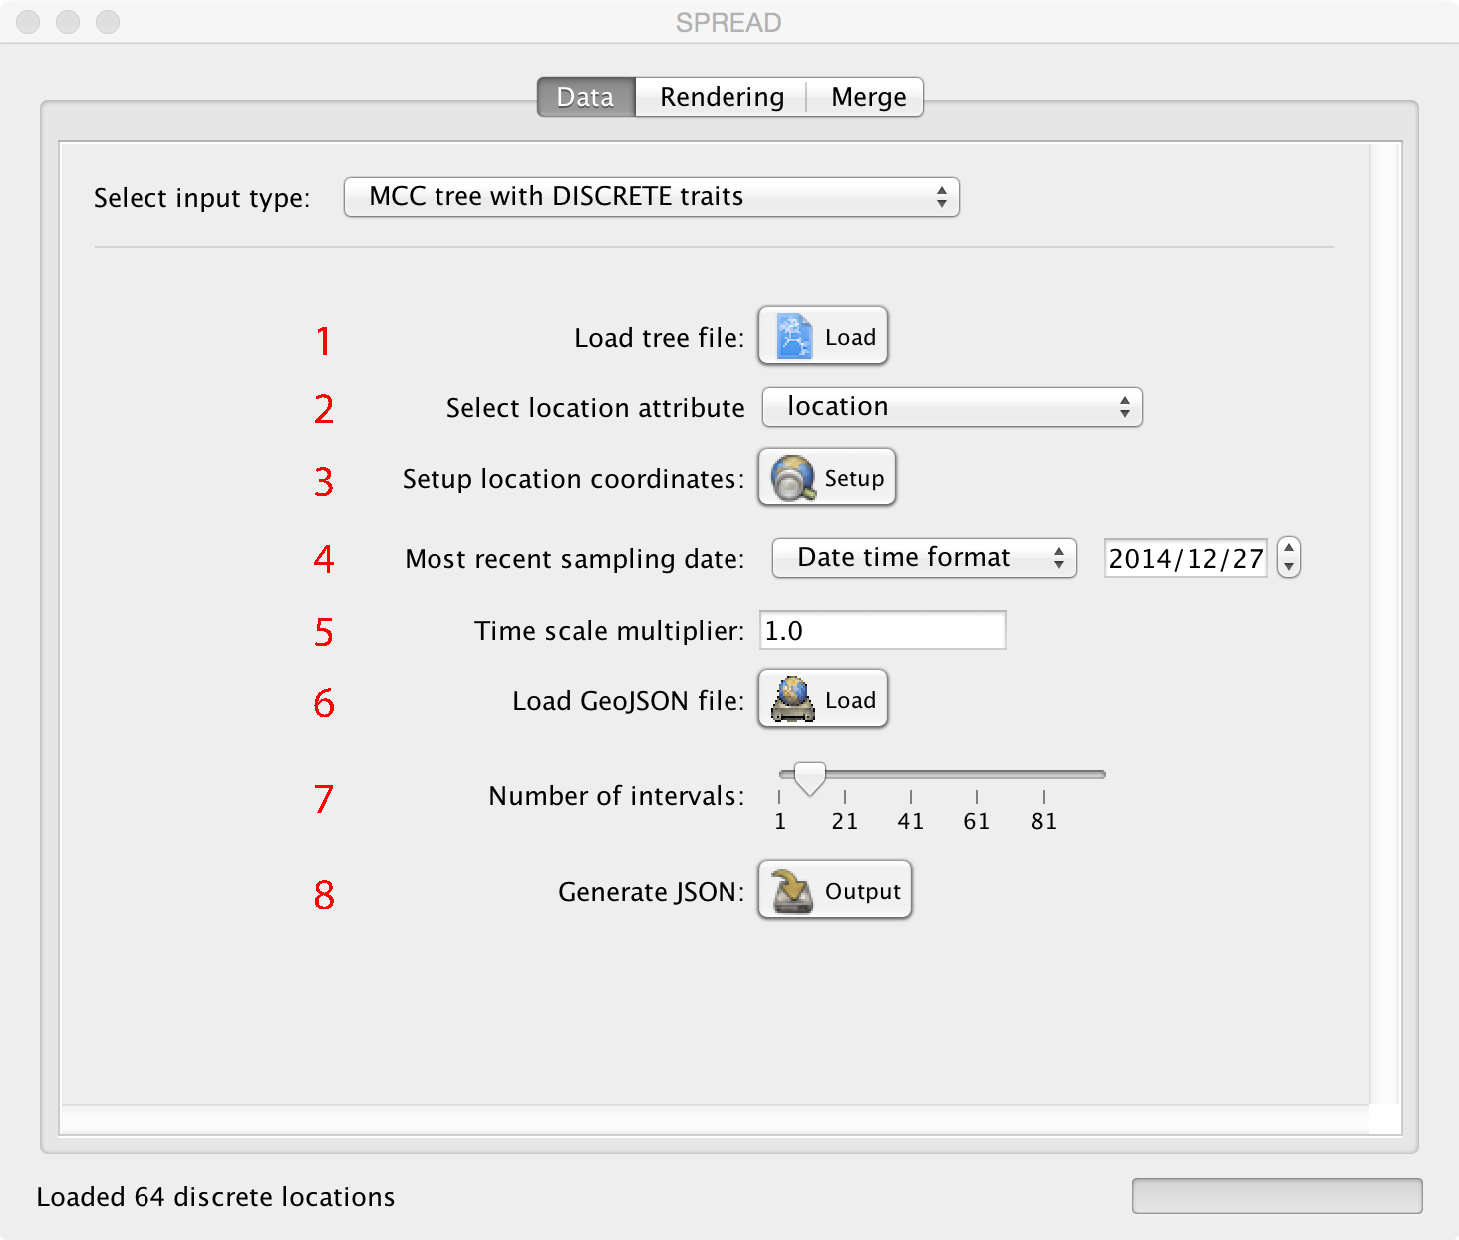
\includegraphics[width=1\textwidth]{./figures/Fig1_parsing_discrete.pdf} %[scale=0.22]
\label{fig:parseDiscrete}
\end{figure}

\subsubsection{Rendering and specifying the visualisation options}

The `Rendering' tab in the GUI by default opens the D3 renderer.
Load `ebov.json' and specify the name of the folder in which the rendered output will be stored. %adjust name in GUI: not 'to' but 'with'
Following the name-giving in Figure \ref{fig:renderD3}, this creates a folder `ebov\_d3' with several files.
The most important one is 'index.html', which can be opened by any modern internet browser by double-clicking. 
\par
The visualisation options can be set via menu's in the left column of the window.
The branches of the tree are represented by lines and the nodes by points. %polygons, circular polygons
Each has particular properties (e.g. color, opacity, \dots) that can either be given a fixed value, or have values assigned by corresponding traits.
\par
`index.html' opens a web-page showing the tree and the sampling locations mapped in their geographical context (Figure \ref{}). 
For this example, let's lay the visual focus on the cross-country location transitions.
Start by colouring the map by country. 
To concentrate on the pure geographical aspect of the picture, unselect the Polygons and Lines layer under `Toggle layer visibility'.
Now set the `Map fill attribute' to 'ISO', which assigns a different color to Guinea, Sierra Leone and Liberia.
Lower the `Map fill opacity' to 0.2 to enhance the contrast with the branch colors (cfr. infra).
Set the size of the `Point area' to 4 and also color the sampling locations by country via the `Point color attribute'.
Reselect the Lines layer.
Setting the `Line color attribute' to `country' colours the lines by destination location, and attracts the eye to cross-country movements.
Reselect the Polygons layer.
Because the size of the polygons around a sampling location is proportional to the number of lineages that are estimated to reside at that location, this captures the relative intensity with which the various locations are affected at any given point in time.
For example, set the `Circular polygon color'  to the darkest red in combination with a low value for its opacity. 
After this, the figure should closely resemble Figure 1a in \cite{Bielejec:2016aa}.

\begin{figure}[!H]
\centering
\includegraphics[width=1\textwidth]{./figures/fig2_render_d3.pdf} %[scale=0.22]
\label{fig:renderD3}
\end{figure}

\begin{figure}[!H]
\centering
\includegraphics[width=1\textwidth]{./figures/fig2_render_d3.pdf} %[scale=0.22]
\label{fig:renderD3}
\end{figure}

\subsection{Visualising a MCC tree annotated with continuous traits}
% 2.3 MCC tree with Continuous traits
%  - languages example would look really nice here overlayed on a whole
% world map
\subsection{Visualising a distribution of trees annotated with continuous traits}
\subsection{Visualising a MCC tree annotated with continuous traits}
\label{JSONmerge}
%combine multiple layers
\subsection{Identifying well-supported rates using Bayes factors test}

% 2.2 BF calculation and visualisation
%  - there seems to be a lot of confusion among folks as to what this
% actually does. I've seen them do calculations on binary coefficients
% other than indicators, or dismiss it thinking we do HME to get the BF
% we could use this to mitigate some of that confusion, so write what
% (and how) do we actually calculate these. I suppose a table in a text
% file is of main use but we also show the (graph) visualisation. H5N1 as
% an example?
% 
% - in location coordinates editor there's now 'generate button that will uniformly spread locations over a circle. Show an example of how this can be used to generate a vis (doesn't need a map layer, so no geojson needed). Perhaps more exciting than just a mere graph of BF values
%
\subsection{Time-slicing}
-> to be put under MCC continuous 

% 2.4 time-slicing 
% - West Nile Virus as an example?
% - show how one can use MCC tree to generate the slices or define
% his/her own slice heights
% - merge continuous tree with JSON file resulting form time slicing a
% posterior distribution for a joint visualisation.
% 
% 

\subsection{Tips \& tricks}
\label{tips}
% Tips & Tricks
%  - we should show the antigenic coordinates example here, where the
% coordinates are other than lat/long and there's no underlying map. I
% also have the multiple HPD's example, on which we can sho whow the
% merging works. W parse 3 JSONs for all HPD levels, merg ethem and
% jointly visualise, coloring polygons by HPD levels.
% - antigenic coord (or any other trait for taht matter) coul dbe plotted as a function of time (height attribute)
% - nodes/ branches of a given tree can be anotated in Figtree, these
%   values can then be used as a basis for mapping
% 
% - Some examples of KML rendering, using previously generated JSON files,
%   just to show that we still support it.

\section{not made up my mind yet on what example to use for the kml rendering}

To create a JSON data file compatible with KML-based rendering, we parse the MCC tree without passing the corresponding geoJSON map as an argument:
\\
\$ spread -parse -locations locations.txt -tree ebov\_mcc.tree -locationTrait location -intervals 10 -mrsd 2015.8 -output ebov\_discrete\_noMap.json
Note that the number of intervals is set to 10, meaning that xxx.
Also note that when nodes are annotated with two or more trait states, SpreaD3 will randomly pick one of these.  
To create the ready-to-use KML file with the default settings, run
\\
\$ spread -render kml -json ebov\_discrete\_noMap.json -output ebov\_discrete\_noMap.kml
\par
meaning of options?
\\-intervals
\\-header T/F
\\
To project annotated trees on a

intervals = time slices; chops the tree in n time intervals => used to calculate for example the counts of a particular transition between states
 
\par
%We provide an over view of the options that the user can specify to fine-tune the appearance of the elements representing the phylogeny, its associated traits and their corresponding uncertainty, namely \textit{points}, \textit{lines} and \textit{counts} in Table \ref{tab:options}.
We provide an over view of the options that the user can specify to fine-tune the appearance of the elements used to represent all facets of the phylogeny and its associated traits, namely \textit{points}, \textit{lines} and \textit{counts} in Table \ref{tab:options}.
\\are these available for the KML AND D3 rendering?

%TABLE 1
\vspace{0.5cm}
\begin{table}[!ht]
\centering
\caption[Overview of the available options]{\footnotesize{\textbf{Overview of the available options}}}
\begin{tabular}{ll}
\\
\toprule
			\multicolumn{2}{c}{points}			\\
\midrule	
								&						\\
\textit{color}:					&						\\
								&						\\
override default points color			& -pointColor 0 255 255										\\
map point colors to a continuous attribute 	& -pointColor 0 255 255 -pointColorMapping location$^\ddagger$\\
%differnentiate point attribute using colors 
map point colors to a discrete attribute:	& 					 									\\
	-same color for all states			&-pointColor 0 255 255 -pointColorMapping location					\\
	-state-specific colors: via color sheet$\dagger$&-pointcolors traitColors.txt -pointColorMapping location		\\
								&						\\
\textit{area}: 					&						\\
								&						\\
%no value to be set?
override default points area			& -pointArea 2000	\\						
map point areas to a continuous attribute	& -pointAreaMapping height									\\
map point areas to a discrete attribute	& -pointAreaMapping location									\\
%resizes point area proportional to max of selected trait values
\midrule
			\multicolumn{2}{c}{lines}			\\
\midrule
								&						\\
\textit{color}:					&						\\
%color lines by destination of discrete trait
								&						\\
override default lines color				&	-lineColor 250 0 0		\\
map line colors to a continuous attribute	&	-lineColor 250 0 0 -lineColorMapping length				\\
map line colors to a discrete attribute:	&						\\
	-same color for all states			&	-lineColor 250 0 0 -lineColorMapping location				\\
	-state-specific colors: via color sheet$\dagger$&-linecolors traitColors.txt -lineColorMapping location		\\
%start color and end color: color changes between these - similar setup for discrte and continuous traits
								&						\\
\textit{width}:					&						\\
								&						\\
	override default lines width		&-lineWidth \textit{number}	\\
								&						\\
								&						\\
\textit{altitude}:				&						\\
%max altitude uniformly applied to all?
								&						\\
override default lines altitude			&-lineAltitude  \textit{number}	\\
%no differentiation in altitude by trait value? 
map line altitude to a continuous attribute	&-lineAltitude  \textit{number} -lineAltitudeMapping height	\\
map line altitude to a discrete attribute	&-lineAltitude  \textit{number} -lineAltitudeMapping country\\
								&						\\
\midrule
			\multicolumn{2}{c}{counts}				\\
\midrule
								&						\\
\textit{color}:					&						\\
								&						\\
override default count color			&	-countColor 0 0 250		\\
								&						\\
\bottomrule
\end{tabular}
\begin{flushleft}
{\footnotesize 
$\dagger$: a file with per line only the trait state name and its color code, separated by a tab. The colors should be supplied in RGB or RGBA values.
\\
$\ddagger$: while here the trait of interest in a standard pylogeographical analysis  typically would be location trait, this can be any discrete trait of choice.
} 
\end{flushleft}
\label{tab:options}
 \end{table}


%in GUI-mode: when rendering, the boxes too large to be visualised in 1 screen - for ease of use I strongly suggest these fit 1 screen. 
%in GUI-mode: default is that tweaking options are not set, I would add this option to the choice list
%GUI: when rendering EBOV, parsed with 'location attribute', selecting point colors 'country', point color 'blue' -> points are still shades of green???
%GUI: when selecting both points color and area coording to Country, there is a Liberia location in the middle of Sierra Leone plus another one near the border. Also one Liberia and several Sierra Leone locations in Guinee??? Artefact of negative branch lengths in MCC tree?
%GUI: lines color is not the selected one??
%GUI line width: seems OK
%GUI area color: not selected choice 
%GUI counts color: seems OK. But I wonder: what makes an area suddenly pop up? Is this the number of intervals -> yep?

LINE COLOR = GET CHILD NODE COLOR




\bibliographystyle{apalike}
\bibliography{tutorefs.bib} 

\end{document}
